\documentclass[12pt,letter]{article}
\usepackage{mathptmx} % added for time new roman font
\usepackage[left=1in,right=1in,top=1in,bottom=1in]{geometry}
\usepackage[latin1]{inputenc}
\usepackage{amsmath}
\usepackage[final]{pdfpages}

\usepackage[textsize=tiny]{todonotes}

% defines all example enviorment
\usepackage[framemethod=tikz]{mdframed} % added for the box around examples
\newtheorem{ex}{Example}
\numberwithin{ex}{section} % allows for the use of example numbers that lign up with the section numbers
\newenvironment{example}{\begin{mdframed}[middlelinewidth=0.5mm]\begin{ex}\normalfont}{\end{ex}\end{mdframed}}

% defines all review enviorment
\usepackage[framemethod=tikz]{mdframed} % added for the box around examples
\newtheorem{re}{Review}
\numberwithin{re}{section} % allows for the use of example numbers that lign up with the section numbers
\newenvironment{review}{\begin{mdframed}[middlelinewidth=2mm,roundcorner=20pt]\begin{re}\normalfont}{\end{re}\end{mdframed}}

% defines the quotation enviorment 
\usepackage{xcolor}
\newcommand{\quotebox}[2]{\begin{center}\fcolorbox{white}{blue!15!gray!15}{\begin{minipage}{0.9\linewidth}\vspace{10pt}\center\begin{minipage}{0.8\linewidth}{\space\Huge``}{#1}{\Huge''}{\break\null\hfill} {\small #2}  \end{minipage}\medbreak\end{minipage}}\end{center}}

% defines the definition enviorment 
\newcommand{\definitionbox}[2]{\begin{center}\fcolorbox{white}{blue!15!gray!15}{\begin{minipage}{0.9\linewidth}\vspace{10pt}\center\begin{minipage}{0.8\linewidth} {{\textbf{Definition} - }{#1}: {#2}}\end{minipage}\medbreak\end{minipage}}\end{center}}

\usepackage{amsfonts}
\usepackage{amssymb}
\usepackage{graphicx}
\usepackage{float}
\usepackage{booktabs}
%\usepackage{parskip} % remove all the paragraph indents
\usepackage{xfrac}
\usepackage{upgreek}
\usepackage{wrapfig}
\usepackage{setspace}
\usepackage[colorlinks=true]{hyperref}
\usepackage{textcomp} 
\usepackage{multicol} 
\usepackage{enumitem}		% added for spacing in itemize lists
\usepackage[numbered,framed]{matlab-prettifier}		% added for matlab code
\let\ph\mlplaceholder % shorter macro
\lstMakeShortInline"
\lstset{
  style              = Matlab-editor,
  basicstyle         = \mlttfamily,
  escapechar         = ",
  mlshowsectionrules = true,
}

\usepackage{color} % color added for editing
\newcommand{\bl}[1]{\textcolor[rgb]{0.00,0.00,1.00}{#1}}
\newcommand{\gr}[1]{\textcolor[rgb]{0.00,0.50,0.00}{#1}}
\newcommand{\rd}[1]{\textcolor[rgb]{0.75,0.00,0.00}{#1}}

\usepackage{fancyhdr}
\pagestyle{fancy}
\fancyfoot{} % clear all footer fields
\fancyfoot[LE,RO]{Page \thepage} 
\fancyfoot[RE,LO]{}

%%%%%%%		define the symbols for positive directions		%%%%%%
\makeatletter													%%	
																%%					
\newcommand*\curveplus{% positive counterclockwise				%%
  \mathbin{\rotatebox[origin=c]{90}{$\m@th\curvearrowleft$}+}}	%%
																%%
\newcommand*\rightplus{% positive right							%%
  \mathpalette\@rightplus\relax}								%%
\newcommand*\@rightplus[1]{%									%%
  \mathbin{\vcenter{\hbox{$\m@th\overset{#1+}{\to}$}}}}			%%
																%%	
\newcommand*\upplus{% positive up								%%
  \mathbin{+\mathord\uparrow}}									%%
																%%			
\newcommand*\downplus{% positive down							%%		
  \mathbin{+\mathord\downarrow}}								%%
  																%%		
\newcommand*\downrightplus{% positive down and right			%%	
  \mathbin{+ \rotatebox[origin=c]{-30}{$\m@th\rightarrow$}}}	%%
\makeatother 													%%	
%%%%%%%%%%%%%%%%%%%%%%%%%%%%%%%%%%%%%%%%%%%%%%%%%%%%%%%%%%%%%%%%%%


\usepackage{mathtools}          %loads amsmath as well added for the piece wise function
\DeclarePairedDelimiter\Floor\lfloor\rfloor
\DeclarePairedDelimiter\Ceil\lceil\rceil

 
\newcounter{NumberInTable}
\newcommand{\LTNUM}{\stepcounter{NumberInTable}{(\theNumberInTable)}}

\newcommand{\Laplace}[1]{\ensuremath{\mathcal{L}{\left[#1\right]}}}
\newcommand{\InvLap}[1]{\ensuremath{\mathcal{L}^{-1}{\left[#1\right]}}}
\renewcommand{\textuparrow}{$\uparrow$}


\numberwithin{equation}{section}	% added so the equsation numbers are section.# and start at section.1

\begin{document}
	
	% set the section number, along with figure and equation numbers
	\setcounter{section}{1}	
	\setcounter{figure}{0}   
	\renewcommand\thefigure{\thesection.\arabic{figure}}


\section{Systems}

	\subsection{Basic Concepts in Vibrations}

    The study of vibrations, within the broader field of classical mechanics, is the investigation of oscillations that occur about an equilibrium point. Vibrations, both desired and undesired, are present in all mechanical systems and can be helpful (e.g. a soil sieve, rotary sander) or destructive (e.g. an aircraft frame in resonance). The oscillations that form a vibrating system may be periodic (e.g., pendulum) or random (e.g. turbulence in an airplane), or a combination of the two. 

    Vibrations impact our daily lives in a variety of ways, from the sound made by banjo strings that vibrates between 140 and 400 Hz to the 4-6 Hz vibration felt by a passenger in a car seat. The consideration of the vibrations and their associated mathematical modeling are an important factor in the design of mechanical systems. In the material that follows, the fundamental theories of vibration are presented and modeled using fundamental physical principles such and Newton's three laws of motion. These models and analyzed using the mathematical tools of calculus and differential equations. 

	\begin{review}
		Newton's three laws of motion:
		\begin{enumerate}
			\item In an inertial frame of reference, an object either remains at rest or continues to move at a constant velocity, unless acted upon by a force.
			\item In an inertial reference frame, the vector sum of the forces $F$ on an object is equal to the mass m of that object multiplied by the acceleration of the object: $F = ma$. (It is assumed here that the mass m is constant)
			\item When one body exerts a force on a second body, the second body simultaneously exerts a force equal in magnitude and opposite in direction on the first body.
		\end{enumerate}
	\end{review}

	\subsection{Single Degree-of-Freedom Systems}
	
        In its simplest form, the phenomenon of vibration is the exchange of energy between potential and kinetic energy. Therefore, a vibrating system must have a component that stores potential energy. This component must also be capable of releasing the energy as kinetic energy. This kinetic energy is stored in the movement of a mass where the measure of this movement is the velocity of the system and the continuous interchange between potential and kinetic energy is the vibration of the system. The simplest vibrating systems can be modeled as a single-degree-of-freedom (1-DOF) system. In a 1-DOF system, one variable can describe the motion of a system. Potential examples of  1-DOF systems include:
		
		\begin{enumerate}
			\item yo-yo
			\item pogo stick
			\item door swinging on axis
			\item throttle (gas pedal)
		\end{enumerate}
				
		\noindent Variables often used for describing 1-DOF systems are $x(t)$,  $y(t)$,  $z(t)$, and  $\theta(t)$.  Examples of 1-DOF systems are presented in figure \ref{fig:Examples_of_1DOF_systems} where the assumption of small displacements is made. Note: we will often drop the ``$(t)$'' for simplicity in this material. 

		\begin{figure}[H]
			\centering
			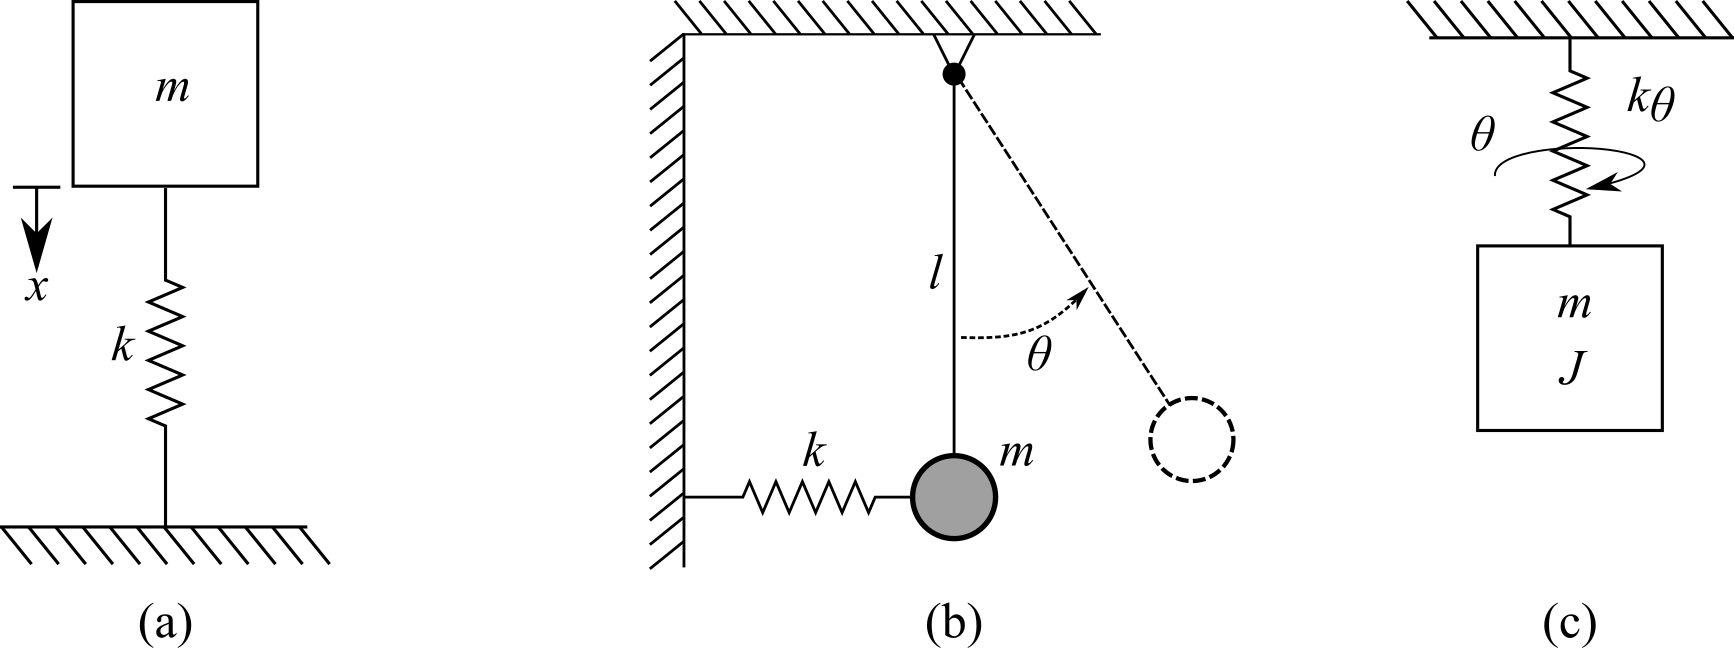
\includegraphics[]{../figures/Examples_of_1DOF_systems.png}
			\caption{Examples of single degree of freedom (DOF) systems showing: (a) a vertical spring-mass system; (b) a simple pendulum; and (c) a rotational spring-mass system.}
			\label{fig:Examples_of_1DOF_systems}
		\end{figure}

		\subsubsection{Spring-Mass Model}

			\quotebox{\Large{All models are wrong, but some are useful}}{George E.P. Box (1919 - 2013)}	
							
            Newtonian physics describes the motion of particles in terms of displacement $x$, velocity $\dot{x}$, and acceleration $\ddot{x}$ vectors. Moreover, from Newton's second law of motion says that the change in the velocity of mass in motion is a product of the force acting on the mass. A simple way to express this phenomenon is though a spring-mass model as presented in figure  \ref{fig:spring_mass_model_with_point_mass}. These spring-mass models neglect the mass of the spring and concentrate all the mass of the system into a single point. Note that in this case the force vector and mass-acceleration vectors lie on the same axis and as such are collinear. Therefore, these vectors can be easily treated as scalers simplifying the math used in the modeling of the system.     

			\begin{figure}[H]
				\centering
				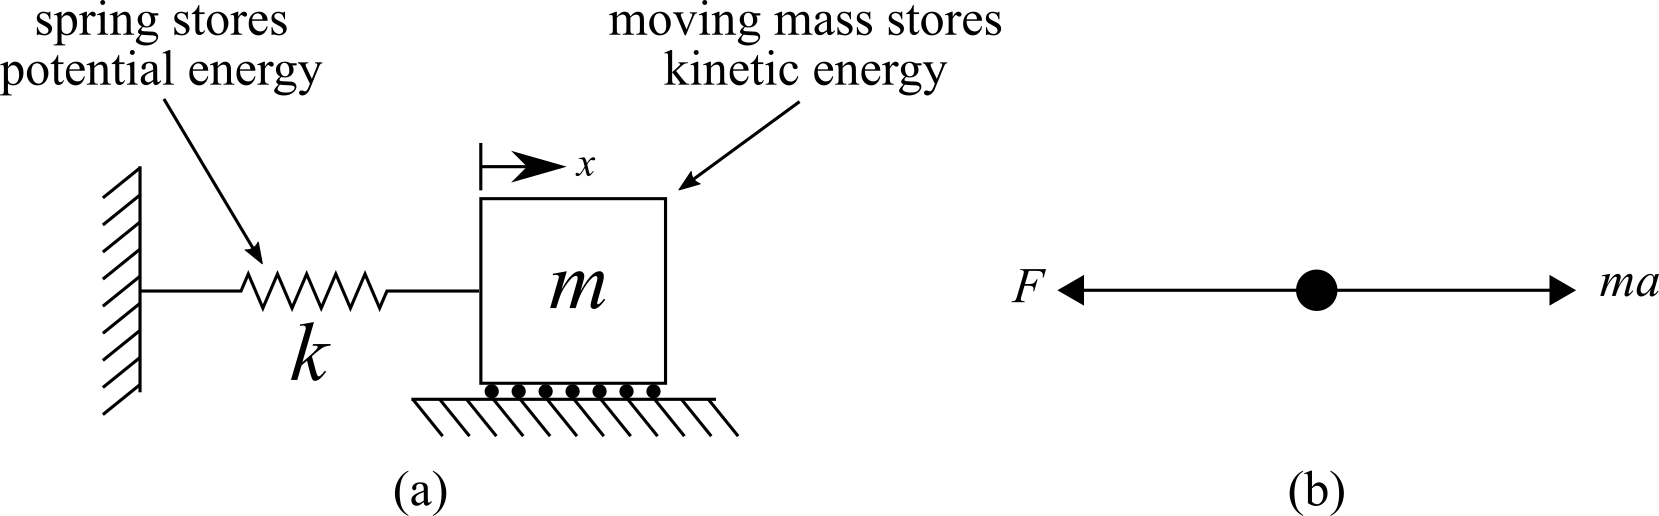
\includegraphics[]{../figures/spring_mass_model_with_point_mass.png}
				\caption{A single-degree-of-freedom (1-DOF) spring mass model showing: (a) annotated schematic of a mass-spring system; and (b) the equivalent free-body diagram represented as a point-mass system.}
				\label{fig:spring_mass_model_with_point_mass}
			\end{figure}	
		
		\subsubsection{Linear Springs}
	
            Springs are mechanical devices that store energy, moreover, ideal spring is a theoretical representation of this mechanical device that is massless and responds with a linear increase in force for a unit increase in displacement (i.e. $F=kx$). For simplicity, the spring in the spring-mass model considered here is assumed aways ideal linear springs. A graphical representation of the idealized linear spring is presented in figure \ref{fig:linear_spring_deformation} where a unit force $F$ applied to the free end of the spring results in a unite displacement $x$ of the spring.  The resulting mathematical relationships,  $F=kx$, is known as Hooke's Law. Nonlinear springs add considerable complexity to the modeling of spring-mass systems, therefore, these are not considered in this introductory work. 
			
			\begin{figure}[H]
				\centering
				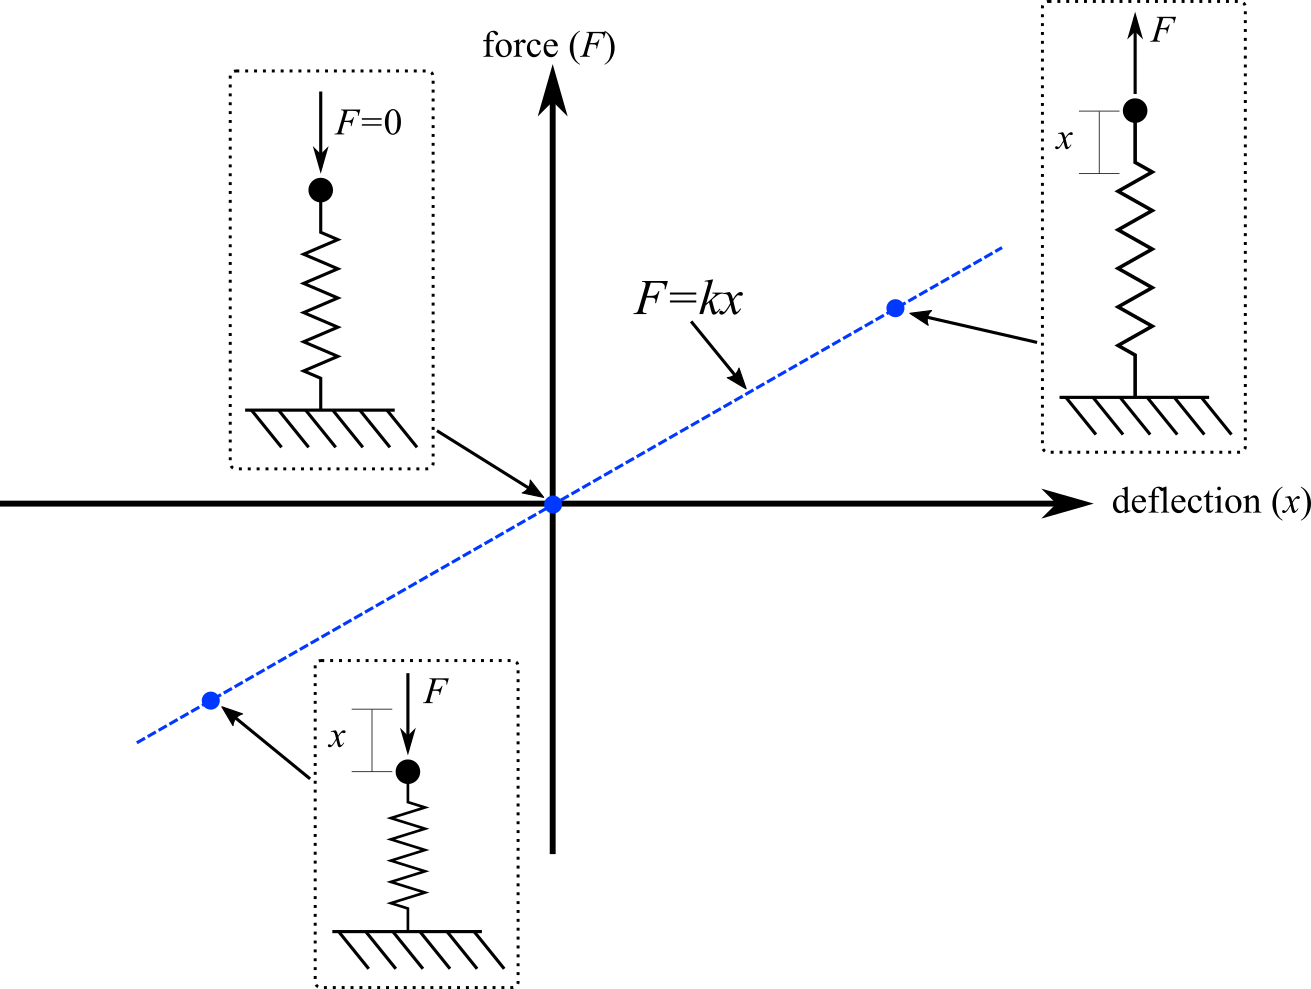
\includegraphics[]{../figures/linear_spring_deformation.png}
				\caption{Force-displacement plot for a linear spring.}
				\label{fig:linear_spring_deformation}
			\end{figure}					






					
	\subsubsection{Equation of Motion for an Oscillating System}			
			
        An Equation of Motion (EOM) is an equation that provides a basis for modeling a vibrating system about its equilibrium point and relates the transfer of the potential energy from the spring to the kinetic energy mass. In developing the EOM we assume that any surfaces are frictionless and as such, no energy is extracted from the vibrating system. Referencing the 1-DOF system in figure \ref{fig:EOM_1-DOF-mass_horizontal}(a), and assuming the mass only moves in the $x$ direction, the only force acting on the mass in the $x$ direction is the force that results from the elongation of the spring as annotated in figure \ref{fig:EOM_1-DOF-mass_horizontal}(b). Therefore, the sum of forces in along the $x$ axis must equal the mass ($m$) times the acceleration of the mass ($a\dot{x}$). 

		\begin{figure}[H]
			\centering
			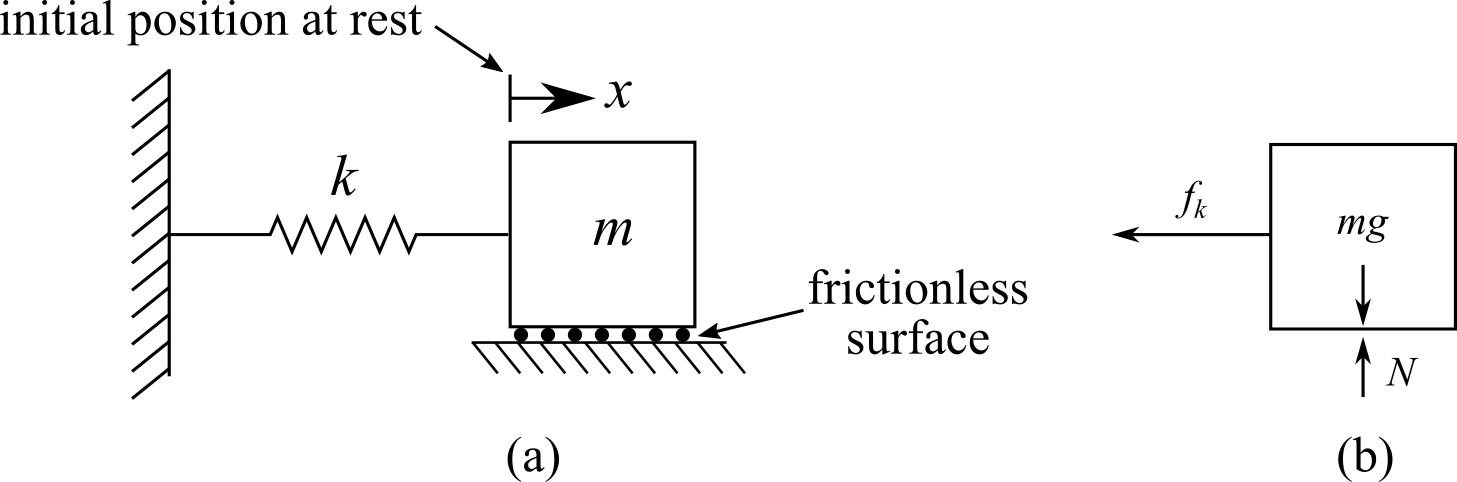
\includegraphics[]{../figures/EOM_1-DOF-mass_horizontal.png}
			\caption{A spring mass model of a 1-DOF system showing: (a) a schematic of the system; (b)  free-body diagram of the system at its initial position.}
			\label{fig:EOM_1-DOF-mass_horizontal}
		\end{figure}			
		
		Considering that positive displacements are to the right, the standard form of the equation of motion for an undamped system without any excitation is expressed as:  
		\begin{equation}
			s_1 \ddot{x} + s_2 x = 0
		\end{equation}			
		where $s_1$ and $s_2$ are constants to be determined for the specific system. A systematic approach to obtaining free-body diagram (FBD) of a system under vibration can be expressed in three steps:
		\begin{enumerate}
			\item Draw a free-body diagram (FBD) at the system's equilibrium and displaced position (without a displacing force).
			\item Apply Newton's second law to both FBDs ( equilibrium and displaced).
			\item Combine the equations to write the EOM in standard form with the forcing component on the right-hand side. For free vibration, the forcing component is 0. 
		\end{enumerate}
			
		Solving these three steps for 1-DOF system presented in figure \ref{fig:EOM_1-DOF-mass_horizontal} results in the EOM:
		\begin{equation}
			m \ddot{x} + k x = 0
		\end{equation}

		\begin{review}
			A second-order linear homogeneous differential equation has the form:
			
			\begin{equation}
			 a \ddot{x} + b \dot{x} + cx = 0
			\end{equation}
		
			\noindent The EOM for a 1-DOF system under a free vibration is a a second-order differential equation due to acceleration ($\ddot{x}$) being the second derivative of displacement ($x$) and homogeneous as the forcing function (right-hand side of the equations) is zero. In EOM's current form, $m=k$, $b=0$,  and $c=k$. In future work, $b$ will account for damping in the vibrating system.     
		\end{review}

					
		\begin{example}			
			
			Considering the system:
			\begin{figure}[H]
				\centering
				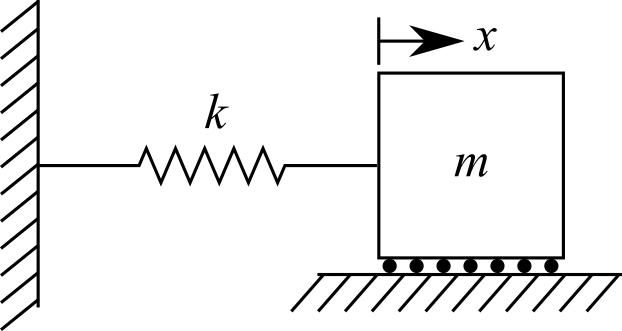
\includegraphics[]{../figures/1-DOF-spring_mass_horizontal.png}
			\end{figure}		
			
			\textbf{Step-1}
			Define the direction of displacement, and draw the FBD for the equilibrium and displaced state.  
			\begin{figure}[H]
				\centering
				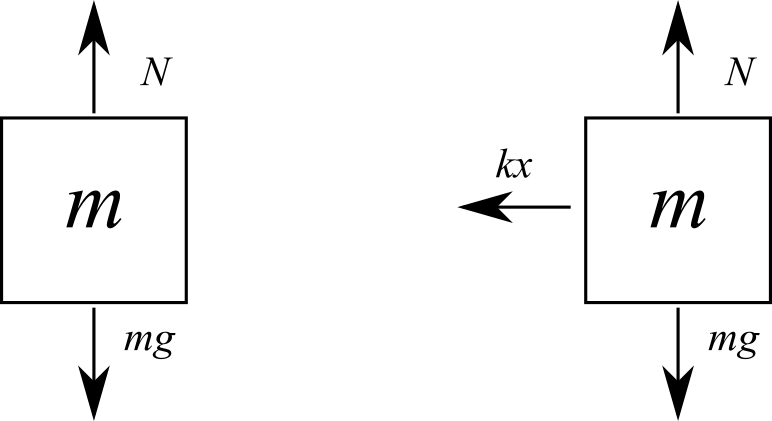
\includegraphics[width=0.45\textwidth]{../figures/1-DOF-mass_horizontal_FBD.png}\\
				equilibrium state \hspace{3cm} displaced state
			\end{figure}		
			\noindent The equation for the equilibrium state is:
			\begin{equation}
			\rightplus \sum F_x = 0
			\end{equation}
			and in the displaced state:
			\begin{equation}
			\rightplus \sum F_x = -kx
			\end{equation}		
			This equation does not equal zero as the FBD does not account for the restoring force. 
	
			\noindent	\textbf{Step-2} Apply Newton's second law (we want to store energy in the kinetic state) of motion to the sum of forces for the displaced position we get: 		 		
			\begin{equation}
			ma = m\ddot{x} = \rightplus \sum F_x = -kx
			\end{equation}			
			\begin{equation}
			m\ddot{x} = -kx
			\end{equation}				
			\textbf{Step-3} Rearrange in the Equation to construct an EOM: 			
			\begin{equation}
			m\ddot{x} + kx = 0
			\end{equation}		
		\end{example}			

		\begin{example}	
			Some systems will have an initial displacement, as the system will oscillate around this position we need to define the EOM about this position. Considering the system:
			\begin{figure}[H]
				\centering
				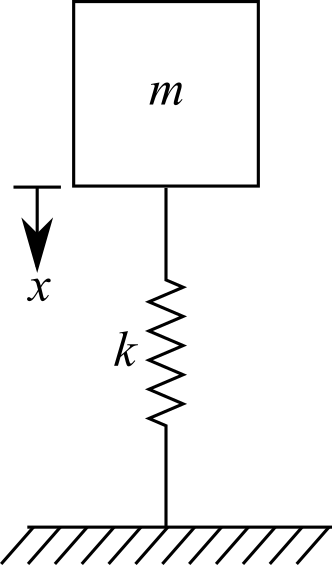
\includegraphics[]{../figures/1-DOF-spring_mass_vertical.png}
			\end{figure}		
			\noindent \textbf{Step-1}
			Define the direction of displacement, and draw the FBD for the equilibrium and displaced state.  
			\begin{figure}[H]
				\centering
				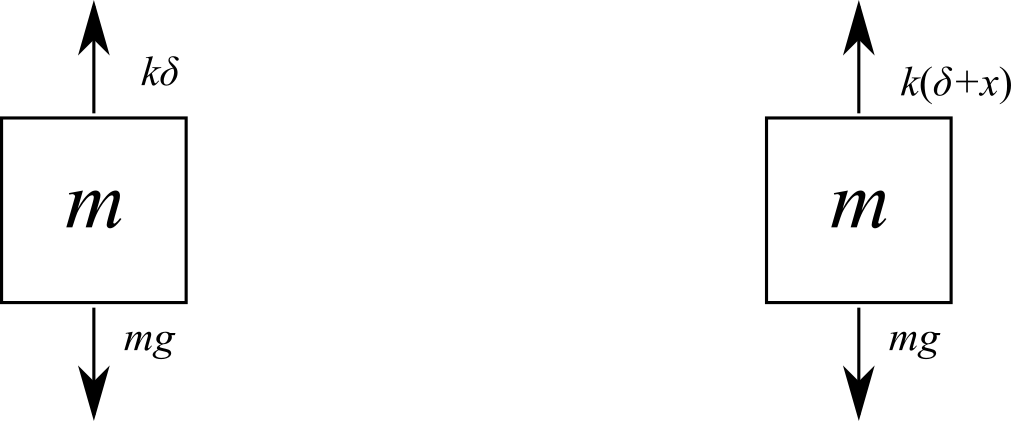
\includegraphics[]{../figures/1-DOF-spring_mass_vertical_FBD.png}\\
				equilibrium state \hspace{3cm} displaced state
			\end{figure}		
			\noindent The equation for the equilibrium state is:
			\begin{equation}
				\downplus \sum F_x = mg - k\delta = 0
			\end{equation}
			and in the displaced state:
			\begin{equation}
				\downplus \sum F_x =mg -k(\delta + x)
			\end{equation}	
			This equation does not equal zero as the FBD does not account for the restoring force.	
			
			\noindent \textbf{Step-2} Apply Newton's second law (we want to store energy in the kinetic state) of motion to the sum of forces for the displaced position we get: 		
			\begin{equation}
				m\ddot{x} = \downplus \sum F_x =mg -k\delta -kx
			\end{equation}
			We can than use the information from the equilibrium state to cancel out some terms, this becomes:
			\begin{equation}
				m\ddot{x} = -kx
			\end{equation}				
			\textbf{Step-3} Rearrange in the Equation to construct an EOM: 					
			\begin{equation}
				m\ddot{x} + kx = 0
			\end{equation}			
		\end{example}	




\subsection{Forcing Function}

\subsubsection{Step Function}

A step function is a common loading situation and can represent the dropping of a load into a truck, a car going over a curve, or a motor starting up. The step function ($\Phi$) is also know as the Heaviside function

\begin{figure}[H]
	\centering
	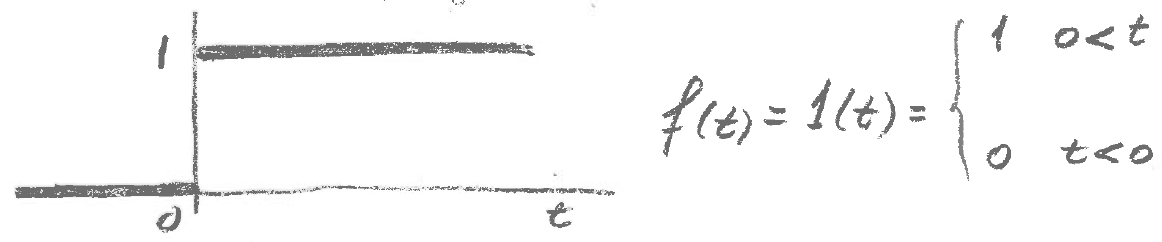
\includegraphics[width=6.5in]{../figures/step.png}
	\caption{Step function.}
\end{figure}



\subsubsection{Pulse Function}

Pulse function ($\rho(t;\uptau)$) consists of a step up at $t=0$ followed by a step down at $t=\uptau$. The amplitude is $\sfrac{1}{\uptau}$ so that the area under the pulse is constant and equal to unity ($A=1$). 

\begin{figure}[H]
	\centering
	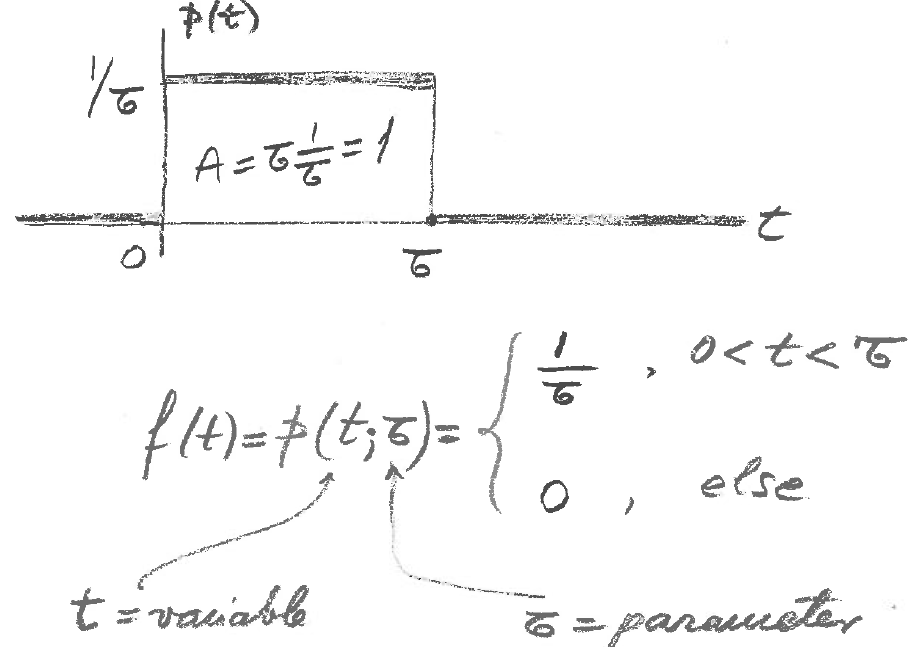
\includegraphics[width=5.5in]{../figures/pulse_function.png}
	\caption{Pulse function.}
\end{figure}

\subsubsection{Impulse Function}

Shock loads on mechanical systems represent a very common source of vibration. These short-duration forces are also called called an impulse. An impulse excitation is defined as a force that is applied for a very short, or infinitesimal, length of time. An impulse is a nonperiodic force that is represented by the symbol $\delta$. Impulse function ($\delta(t)$) is also known as the ``Dirac function'', ``Dirac delta function'', ``Dirac impulse function'', or ``delta function''. The impulse function $\delta(t)$ is obtained from the pulse function $\rho(t;\uptau)$ by letting $\uptau$ become infinitesimally small, i.e., 

\begin{figure}[H]
	\centering
	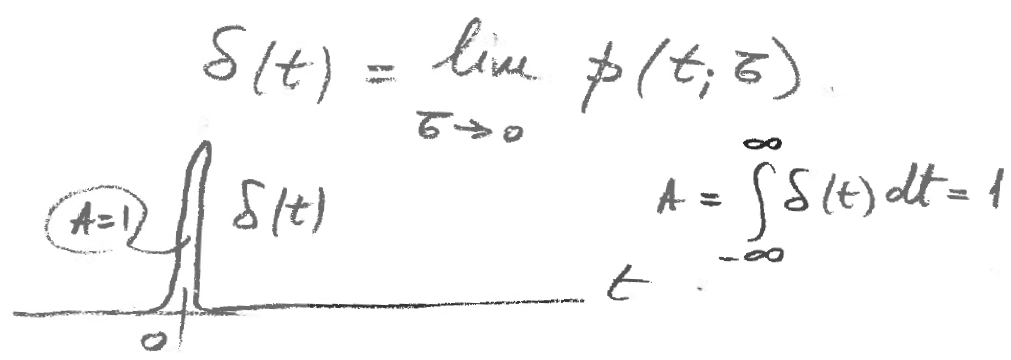
\includegraphics[width=5.5in]{../figures/impulse_function.png}
	\caption{Impulse function.}
\end{figure}

The area under the $delta$ function is equal to unity ($A=1$) just like the pulse function $\rho(t;\uptau)$.

\subsubsection{Ramp Function}

The ramp function is zero for $t<0$ and equal to $t$ for $t>0$. 

\begin{figure}[H]
	\centering
	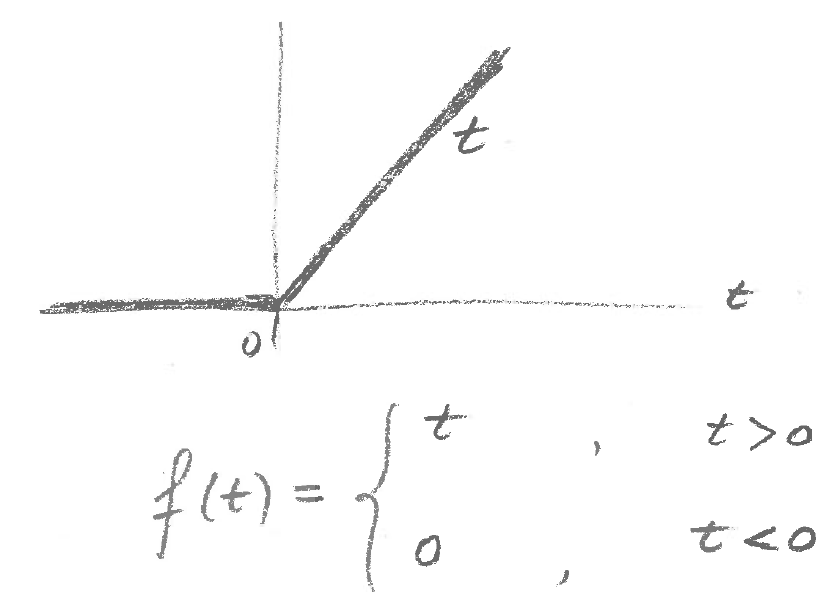
\includegraphics[width=3.5in]{../figures/ramp_function.png}
	\caption{Ramp function.}
\end{figure}



	\subsection{Introduction to Stability}

	The stability of a system is explained though ``poles'' and ``zeros''. The poles and the zeros of a system determine whether the system is stable, and how well the system performs.

	\begin{enumerate}
		\item A system at a pole has an output that is infinite even though the input to the system was finite (i.e. unstable). 
		\item A system at a zero has an output that is finite even though the input to the system was infinite (i.e. stable).
	\end{enumerate}
 








			\begin{figure}[H]
				\centering
				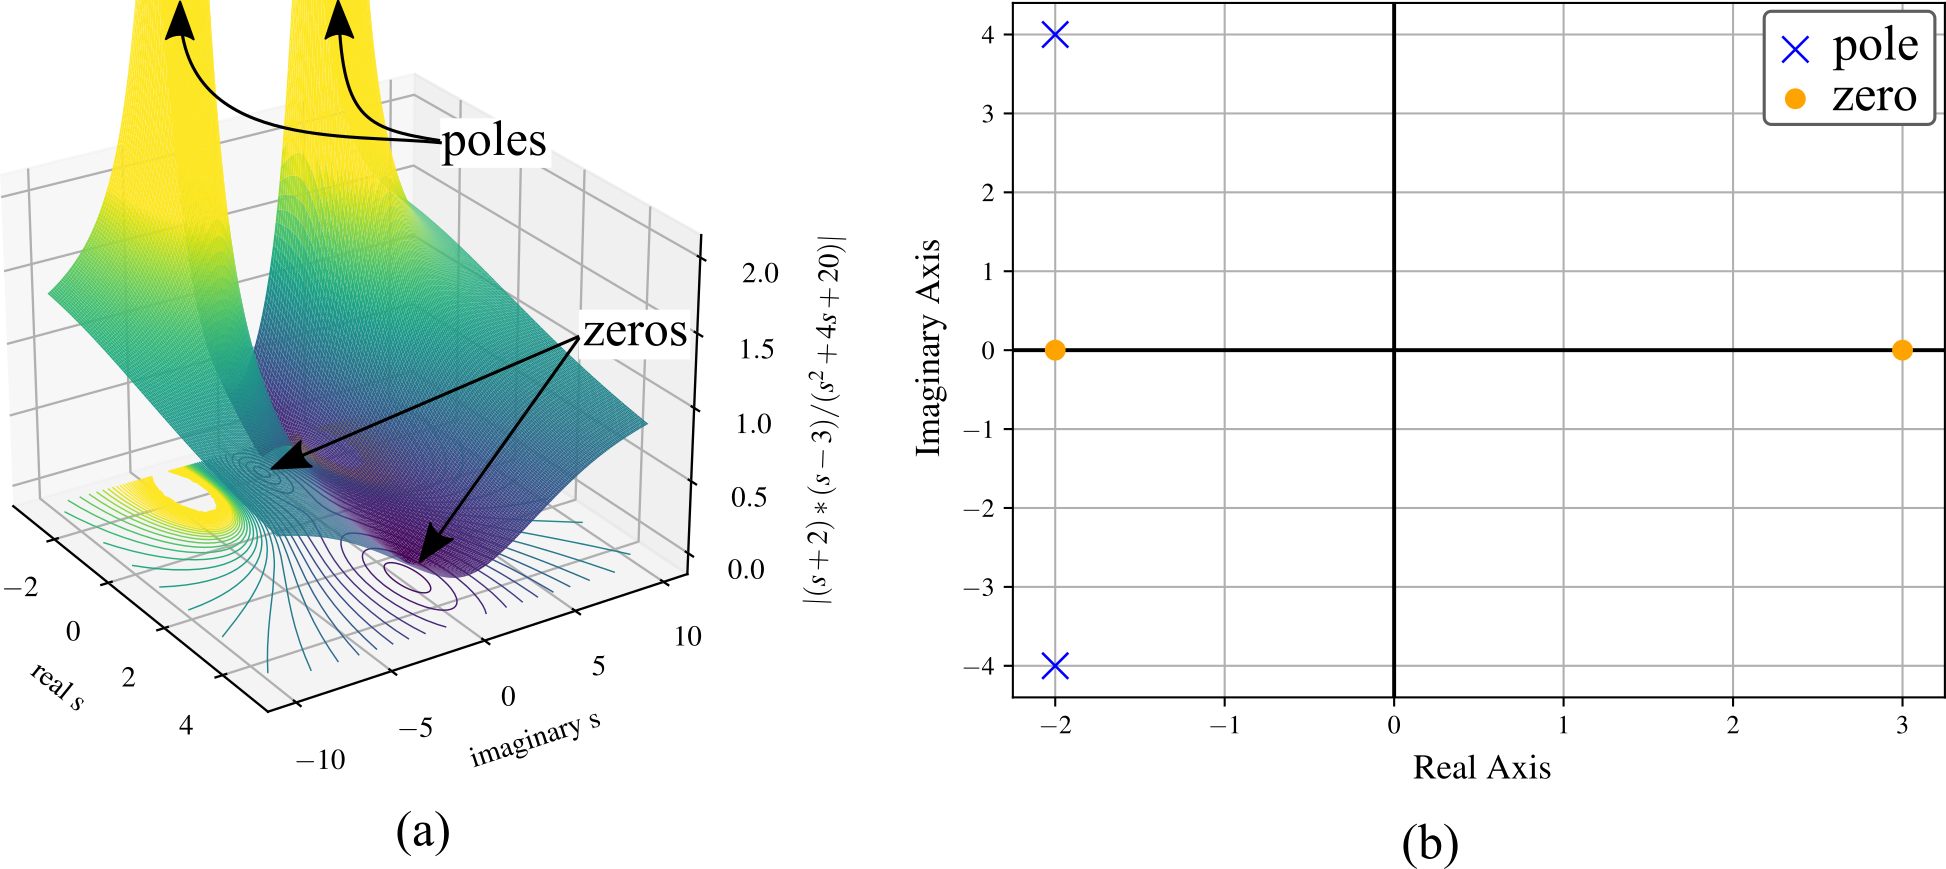
\includegraphics[width=5.0in]{../figures/transfer_function_poles_and_zeros_and_3D_space.png}
				\caption{Poles and zeros.}
				\label{fig:transfer_function_poles_and_zeros_and_3D_space}
			\end{figure}

	Control systems can be designed simply by assigning specific values to the poles and zeros of the system. Physically realizable control systems must have a number of poles greater than the number of zeros. Systems that satisfy this relationship are called Proper. For a rational polynomial transfer function: The poles of a transfer function are defined as the roots of the denominator polynomial of the transfer function.  The zeros of a transfer function are simply the roots of the numerator polynomial. Visualizing of poles and zeros in the complex space can be helpful in understanding the stability of the system. Figure~\ref{fig:transfer_function_poles_and_zeros_and_3D_space} shows the complex space for an arbitrary transfer function $\sfrac{(s+2)(s-3)}{s^2+4s+20}$ where figure~\ref{fig:transfer_function_poles_and_zeros_and_3D_space}(a) shows the 3D space while figure~\ref{fig:transfer_function_poles_and_zeros_and_3D_space}(b) just reports the poles and zeros of the transfer function.  Figure~\ref{fig:transfer_function_3D_space_3_examples} reports the transfer functions for 3 additional transfer functions.  

			\begin{figure}[H]
				\centering
				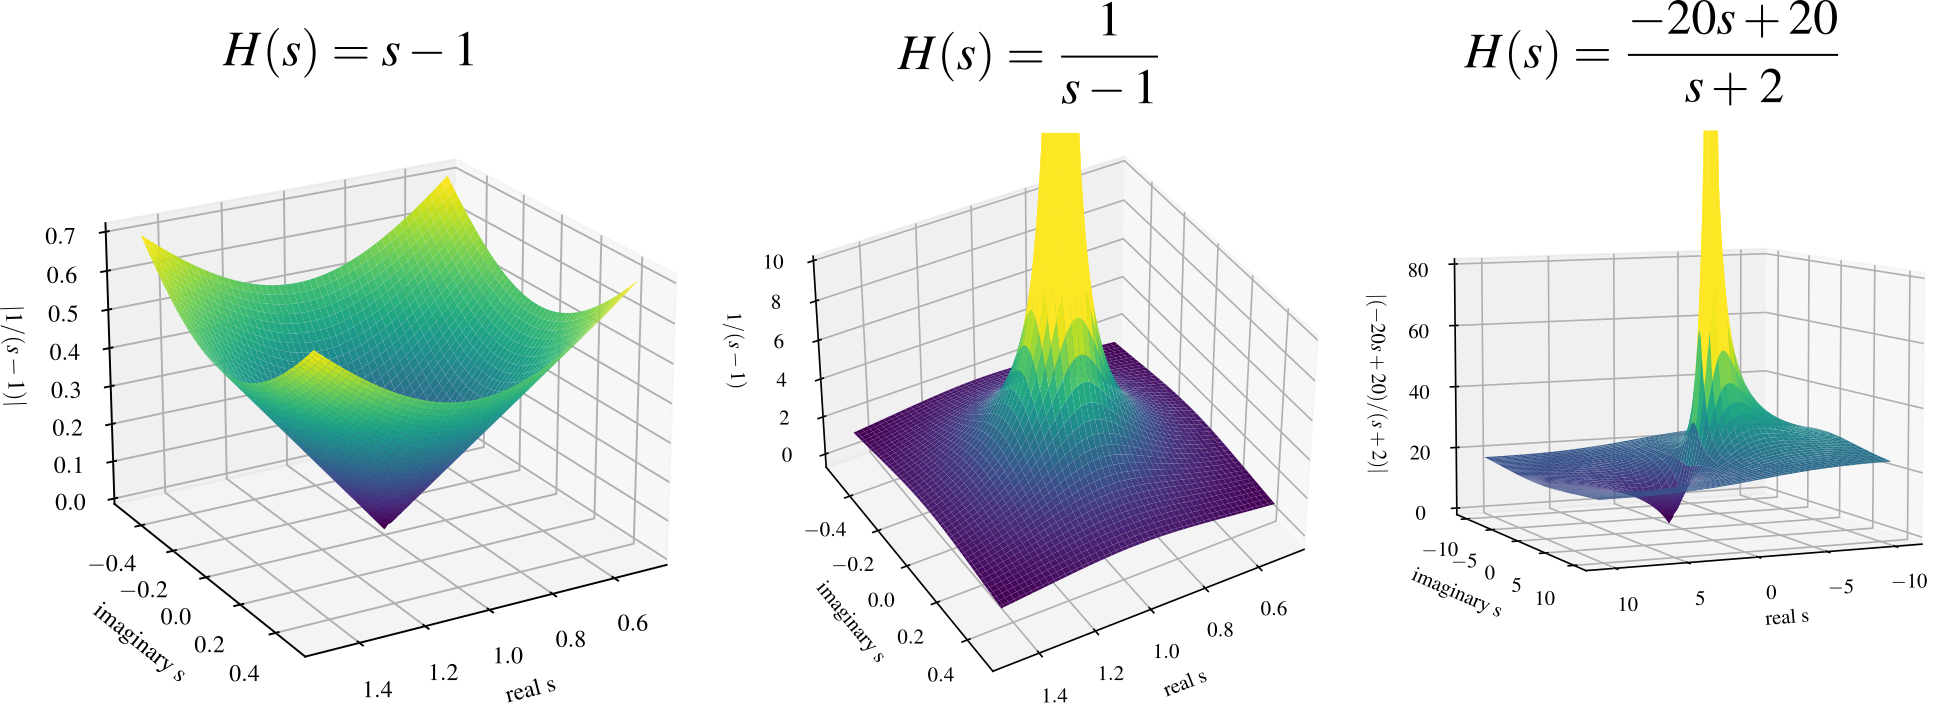
\includegraphics[width=6.5in]{../figures/transfer_function_3D_space_3_examples.png}
				\caption{Poles and zeros in the complex space, plotted for 3 transfer functions.}
				\label{fig:transfer_function_3D_space_3_examples}
			\end{figure}





	\subsection{1\textsuperscript{st} Order Systems}	




	\subsubsection{Spring-damper mechanism}


Consider the system:
\begin{figure}[H]
	\centering
	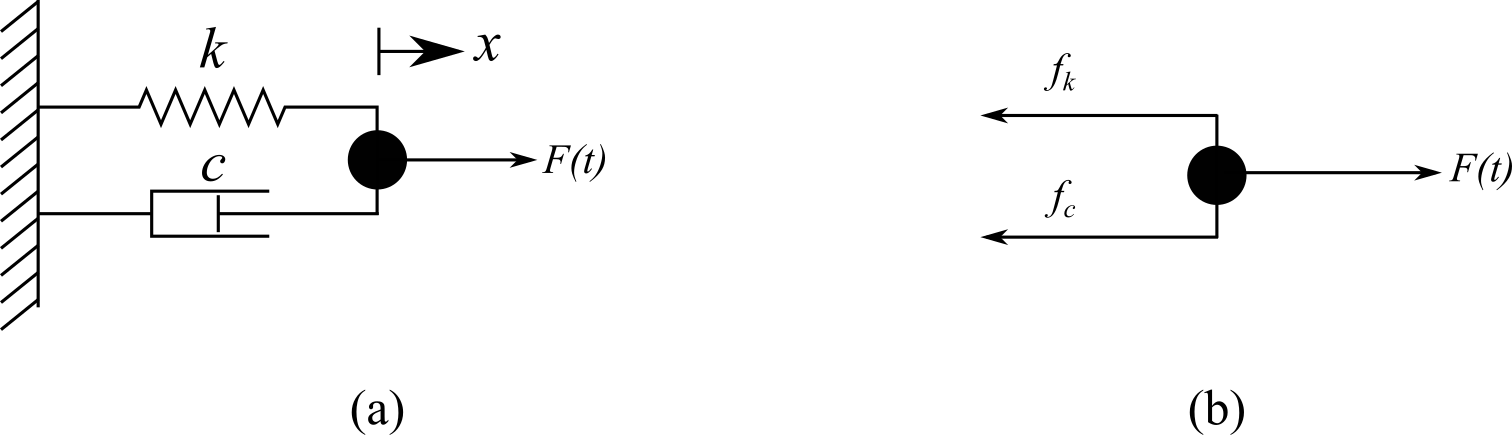
\includegraphics[]{../figures/1-DOF-spring_dashpot_horizontal_forced_FBD.png}
	\caption{Damped 1-DOF system with an external force ($F(t)$) applied, showing: (a) the system configuration; and (b) the free body diagram}
\end{figure}	
Making the assumption that this system does not have any mass, the force balance equation is written as: 
\begin{equation}
-kx - c\dot{x} + f^* =0
\end{equation}
this becomes the equation of motion
\begin{equation}
c\dot{x} + kx = f^*
\end{equation}
normalizing the equation of motion by the stiffness $k$, 
\begin{equation}
\frac{c}{k}\dot{x} + x = \frac{1}{k}f^*
\end{equation}
define the \emph{time constant} $T$ as 
\begin{equation}
T=\frac{c}{k}
\end{equation}
and the normalized forcing function $f(t) = \frac{1}{k}f^*(t)$. This results in the 1\textsuperscript{st}-order ODE in standard form:
\begin{equation}
T\dot{x}(t) + x(t) = f(t)
\label{eq:ODE}
\end{equation}
A general solution for this ODE is written as:
\begin{equation}
x(t) = x_\text{c}(t)+x_\text{p}(t)
\label{eq:ODE_solution}
\end{equation}
where: $x_\text{c}$ is called the ``complementary solution'' and satisfies the homogeneous equation and satisfies the homogeneous equation 
\begin{equation}
T\dot{x}_\text{c} + x_\text{c} = 0
\end{equation}
The homogeneous equation is obtained from equation~\ref{eq:ODE} by making zero the right had side.  The complementary solution $x_\text{c}$ is the free response.

$x_\text{p}(t)$  is called the ``particular solution'' and is used to satisfy the right-hand side of equation~\ref{eq:ODE}. Substituting equation~\ref{eq:ODE_solution} into equation~\ref{eq:ODE} yields:

\begin{equation}
T(\dot{x}_\text{c} + \dot{x}_\text{p}) + x_\text{c}+x_\text{p} = f(t)
\end{equation}
or
\begin{equation}
T\dot{x}_\text{c} + x_\text{c} + T \dot{x}_\text{p} + x_\text{p} = f(t)
\end{equation}
As $T\dot{x}_\text{c} + x_\text{c}=0$:
\begin{equation}
T \dot{x}_\text{p} + x_\text{p} = f(t)
\end{equation}
This shows that:
\begin{itemize}
\item $T\dot{x}_\text{c} + x_\text{c}$ is the solution to the free response.
\item $T \dot{x}_\text{p} + x_\text{p}$ is the solution to the forced response.
\end{itemize}

\subsubsection{Homogeneous Equation (Free Response)}

The Homogeneous equation is obtained from equation~\ref{eq:ODE} and setting the right had side to zero:
\begin{equation}
T\dot{x}_\text{c} + x_\text{c} = 0
\label{eq:homogenous_solution}
\end{equation}
To solve, assume: \todo{I really think $c$ should be $a$ or it confuses with damping.}
\begin{align}
\label{eq:lambda}
x_\text{c}(t) &= c e^{ p t} \\
\dot{x}_\text{c}(t) &= p c e^{ p t} \nonumber
\end{align}
Inserting equation~\ref{eq:lambda} into equation~\ref{eq:homogenous_solution} gives:
\begin{equation}
T (p c e^{ p t}) + c e^{ p t} = 0
\end{equation}
canceling out like terms results in the ``characteristic equation'':
\begin{equation}
T p  + 1 = 0
\label{eq:characteristic_equation}
\end{equation}
therefore:
\begin{equation}
p  = \frac{-1}{T}
\label{eq:pole}
\end{equation}
where this is a ``pole'' of the system. Inserting equation~\ref{eq:pole} into equation~\ref{eq:lambda} results in the ``free response'' of the system:
\begin{equation}
\label{eq:free_response}
x_\text{c}(t) = c e^{ \sfrac{-t}{T}}
\end{equation}
as shown in figure~\ref{fig:1-DOF_free_decay}. Note that the lack of mass in the system prevents it from oscillate as there is no way for it to hold kinetic energy, and therefore no way for it to exchange energy between potential and kinetic forms. 
\begin{figure}[H]
	\centering
	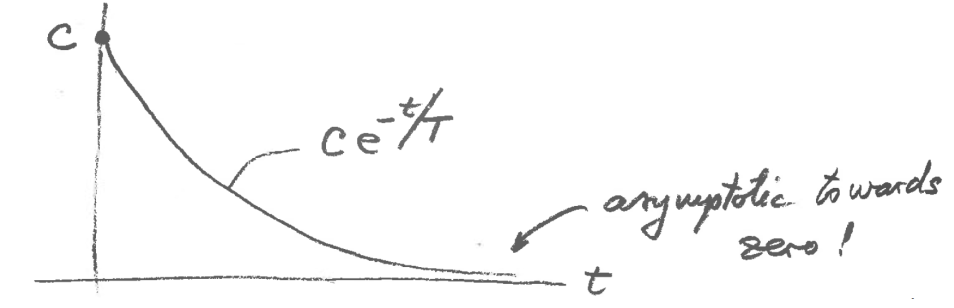
\includegraphics[width=4in]{../figures/free_decay.png}
	\caption{Free decay of a 1-DOF system}
	\label{fig:1-DOF_free_decay}
\end{figure}

\subsubsection{Stability of 1\textsuperscript{st}-order systems}
Using the general free response form eq~\ref{eq:free_response} where $p$ is a root of the charismatic equation (equation~\ref{eq:characteristic_equation}) and is called the ``pole''. The stability of the system is dictate by the sign of of $p$, i.e., its location in the complex $p$ plane.

\begin{mdframed}[middlelinewidth=0.5mm]
\begin{center}
\bl{NOTE}
\end{center}
A \textbf{Stable System} is a system where if a disturbance is applied, then the system returns to its initial state. 
\end{mdframed}

\begin{figure}[H]
	\centering
	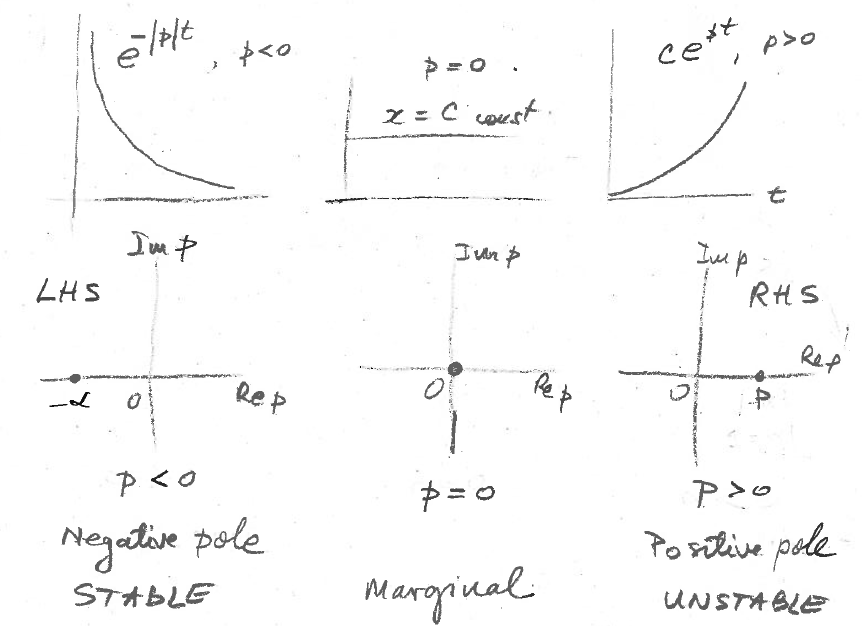
\includegraphics[width=6.5in]{../figures/system_stability_first_order.png}
	\caption{Stability of a first order system for different $p$ values.}
\end{figure}


\subsubsection{Stability of 1\textsuperscript{st}-order Systems Under Forced Response}


The total solution of equation~\ref{eq:ODE} is given as:
\begin{equation}
x(t) = x_\text{c}(t)+x_\text{p}(t)
\end{equation}
or as:
\begin{equation}
x(t) = c e^{ \sfrac{-t}{T}} + x_\text{p}(t)
\end{equation}
The constant $c$ and the function $x_\text{p}(t)$ have to be determined depending on initial conditions and the forms of $f(t)$. In control theory, the initial conditions are usually assumed go be zero. 

\todo{This is incomplete and needs more context.}



\subsection{2\textsuperscript{nd} Order Systems}


Consider the system:
			\begin{figure}[H]
				\centering
				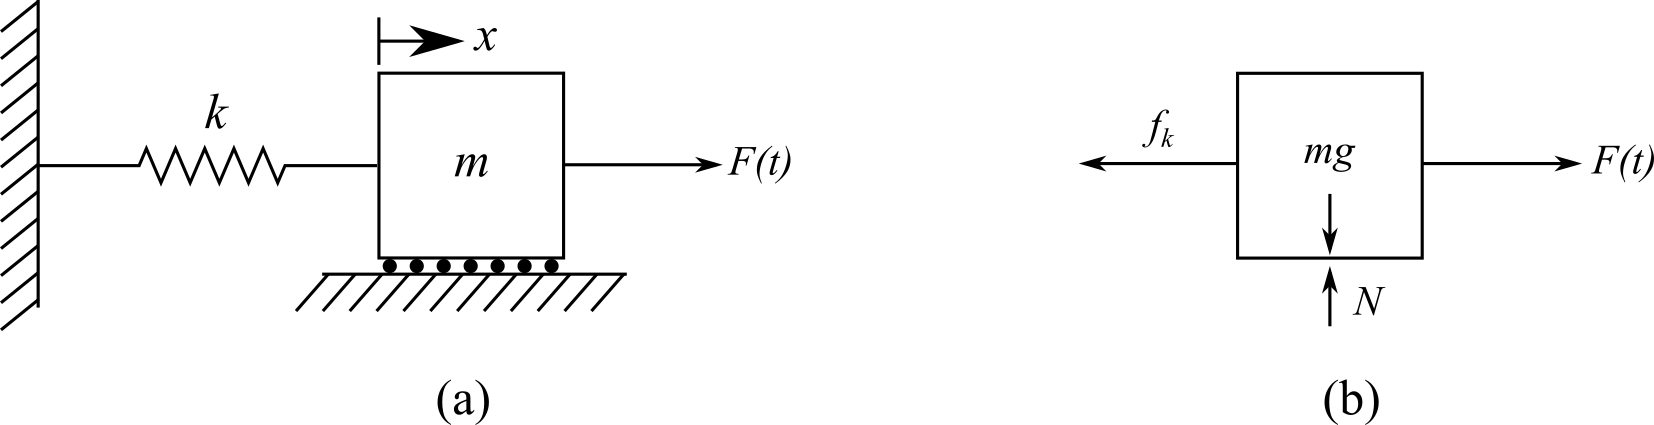
\includegraphics[]{../figures/1-DOF-spring_mass_horizontal_forced_FBD.png}
				\caption{1-DOF system with an external force ($F(t)$) applied, showing: (a) the system configuration; and (b) the free body diagram}
				\label{fig:1-DOF-spring_mass_horizontal_forced_FBD}
			\end{figure}	

Newton's second law of motion states:
\begin{equation}
m \ddot{x} = -k + f^*
\end{equation}
this can be rearranged to the standard equation of motion for a system with forced vibrations:
\begin{equation}
m \ddot{x}(t) + kx(t) = f^*
\label{eq:EOM_2nd}
\end{equation}
It is an 2\textsuperscript{nd}-order inhomogeneous ordinary differential equation in time $t$.  Similar to the solutions to the EOM for a 1\textsuperscript{st}-order system, the solution for a 2\textsuperscript{nd}-order system ae made of two parts, the ``complementary solution'' and the ``particular solution''. Again, this is written as:
\begin{equation}
x(t) = x_\text{c}(t)+x_\text{p}(t)
\end{equation}
where $x_\text{c}(t)$ satisfies the homogeneous equation ($m \ddot{x}(t) + kx(t) = 0$) and represent the ``free'' response of the system. $x_\text{p}(t)$ satisfies the complete equation $m \ddot{x}(t) + kx(t) = f^*$ and represents the ``forced'' response of the system.


\subsubsection{Homogeneous Equation (Free Vibration Response)}

The homogeneous equation $x_\text{c}(t)$ is obtained by setting the forcing function of the EOM to zero:
\begin{equation}
m \ddot{x}(t) + kx(t) = 0
\end{equation}
normalizing by the mass returns:
\begin{equation}
\ddot{x}(t) + \frac{k}{m}x(t) = 0
\end{equation}
denoting the natural frequency of the system:
\begin{equation}
\omega_\text{n}^2 = \frac{k}{m}
\end{equation}
or more simply (and traditionally)
\begin{equation}
\omega_\text{n} = \sqrt{\frac{k}{m}}
\end{equation}
Inserting the natural frequency of the system back into the EOM yields the homogeneous equation in standard form:
\begin{equation}
\ddot{x} + \omega_\text{n}^2 x = 0
\end{equation}
To solve the homogeneous equation, assume the form:
\begin{equation}
x\text(t) = c e^{ p t} 
\end{equation}
hence
\begin{align}
\dot{x}(t)&= p c e^{ p t}  = px\\
\ddot{x}(t)&= p^2 c e^{ p t} = p^2x \nonumber
\end{align}
inserting these back into the EOM for the 2\textsuperscript{nd}-order system results in:
\begin{equation}
 p^2x + \omega_\text{n}^2 x = 0
\end{equation}
this simplifies to the characteristic equation:
\begin{equation}
 p^2 + \omega_\text{n}^2 = 0
\end{equation}
Rearranging this equations lead to
\begin{equation}
 p^2  = -\omega_\text{n}^2
\end{equation}
and considering that $i=\sqrt{-1}$ to the solution
\begin{equation}
p_{1,2}  = \pm i \omega_\text{n}
\end{equation}
inserting these back into the EOM for the 2\textsuperscript{nd}-order system results in:
\begin{equation}
x_\text{c}(t) = c_1 e ^{i \omega_\text{n} t} + c_2 e ^{-i \omega_\text{n} t} 
\end{equation}
which is the the complementary solution where $c_1$ and $c_2$ are constants to be determine.  The complementary solution can also be written as:
\begin{equation}
x_c(t) = c \sin(\omega_\text{n} t + \phi) 
\end{equation}
where $c$ is the amplitude of oscillation and $\phi$ is the phase angle. 

\begin{figure}[H]
	\centering
	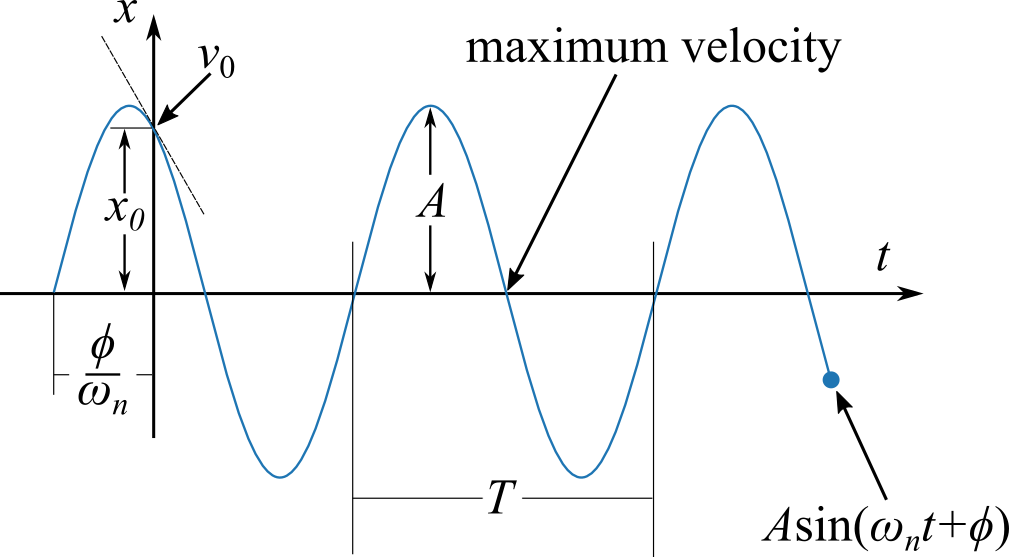
\includegraphics[]{../figures/harmonic_motion_2.png}
	\caption{Summary of the temporal response for a 1-DOF system.}
	\label{fig:Harmonic_Motion_2.png}
\end{figure}
\noindent where $x_0$ and $v_0$ are the is the displacement and velocity at $t$=0 (i.e. the initial displacement). 

		\begin{review}
		
			Euler's (pronounced oy-ler) formula, named after Swiss engineer and mathematician Leonhard Euler (1707-1783), is a mathematical formula in complex analysis that establishes the fundamental relationship between the trigonometric functions and the complex exponential function. Euler's formula states that for any real number $x$,
			\begin{equation}
				e^{j\psi} = \text{cos}(\psi) + j \text{sin}(\psi)
			\end{equation}		
			where $j=\sqrt{-1}$. This equation can also be expressed as:
			\begin{equation}
				e^{-j\psi} = \text{cos}(\psi) - j \text{sin}(\psi)
			\end{equation}	
			This can be expressed in terms of polar coordinates as:				
			\begin{figure}[H]
				\centering
				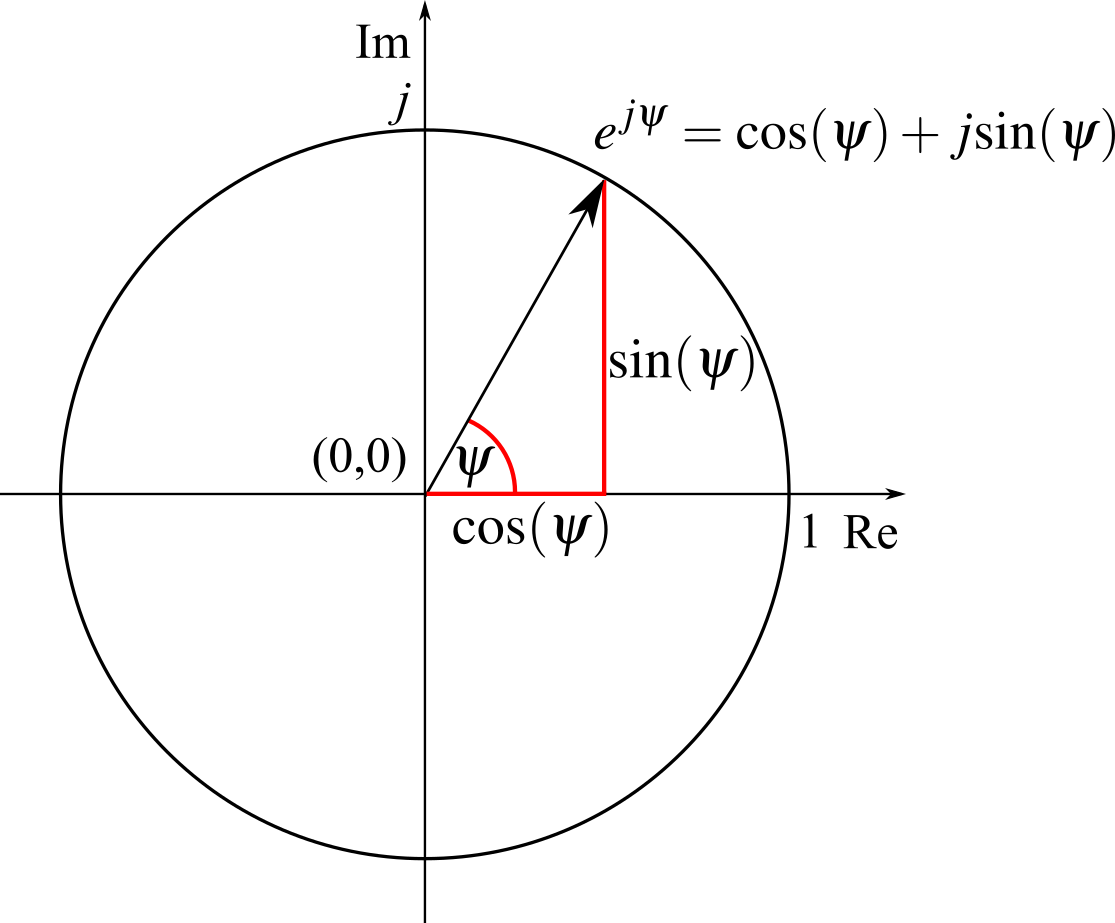
\includegraphics[]{../figures/Eulers_formula.png}
				\caption{Euler's formula illustrated on the unit circle in the complex plane.}
			\end{figure}
		\end{review}


\begin{mdframed}[middlelinewidth=0.5mm]
\begin{center}
\gr{Proof}
\end{center}
Showing that $x_\text{c}(t) = c_1 e ^{i \omega_\text{n} t} + c_2 e ^{-i \omega_\text{n} t} $ is the same as $x_c(t) = C \sin(\omega_\text{n} t + \phi) $, consider Euler's identity, 
\begin{equation}
e^{i \alpha} = \cos(\alpha) + i \sin(\alpha)
\end{equation}
therefore:
\begin{align}
c_1 e ^{i \omega_\text{n} t}   &= c_1 \cos(\omega_\text{n} t) + c_1 i \sin(\omega_\text{n} t)  \\
c_2 e ^{- i \omega_\text{n} t}   &= c_2 \cos(\omega_\text{n} t) + c_2 i \sin(\omega_\text{n} t)   \nonumber
\end{align}
rearranging terms yields:
\begin{equation}
c_1 e ^{i \omega_\text{n} t} + c_2 e ^{- i \omega_\text{n} t}  = (c_1+c_2) \cos(\omega_\text{n} t) + (c_1+c_2) i \sin(\omega_\text{n} t) 
\end{equation}
which is equivalent to:
\begin{equation}
c_1 e ^{i \omega_\text{n} t} + c_2 e ^{- i \omega_\text{n} t}  = A \cos(\omega_\text{n} t) + B \sin(\omega_\text{n} t) 
\end{equation}
where:
\begin{equation}
A = c_1 + c_2; \;\; B = i(c_1 - c_2)
\end{equation}


Recall that $\sin(\alpha + \beta) = \sin(\alpha) \cos(\beta) + \cos(\alpha) \sin(\beta)$. Therefore, $x_c(t) = c \sin(\omega_\text{n} t + \phi)$ can be written as (with a little rearranging):
\begin{equation}
x_\text{c}(t) = c \cos(\phi) \sin(\omega_\text{n} t) + c \sin(\phi) \cos(\omega_\text{n} t)
\end{equation}
Therefore we can show that: 
\begin{equation}
A \cos(\omega_\text{n} t) + B \sin(\omega_\text{n} t) = c \sin(\omega_\text{n} t + \phi) 
\end{equation}
as
\begin{equation}
B = c\cos(\phi); \;\; A = c\sin(\phi)
\end{equation}
Moreover, 
\begin{equation}
A^2 + B^2 = C^2 \sin^2(\phi) + C^2 \cos^2(\phi) = C^2 \big(  \sin^2(\phi) + \cos^2(\phi)\big) = C^2
\end{equation}
and 
\begin{equation}
C = \sqrt{A^2 + B^2}, \;\;\;\;  \frac{A}{B} = \frac{c \sin(\phi)}{c \cos(\phi)} = c \tan(\phi), \;\;\;\;  \phi = \tan^{-1} \frac{A}{B}
\end{equation}

\end{mdframed}

The Standard form of Inhomogeneous Equation can be found, starting at the EOM:
\begin{equation}
m \ddot{x} + kx = f^*
\end{equation}
divide by $m$, therefore:
\begin{equation}
\ddot{x} + \frac{k}{m}x = \frac{1}{m}f^*
\end{equation}
Recall that $\frac{k}{m} = \omega_\text{n}^2$ and define the normalized forcing function as $f(t) = \frac{1}{k}f^*$, this results in:
\begin{equation}
\frac{1}{m}f^*(t) = \frac{1}{m}kf(t) = \omega_\text{n}^2 f(t)
\end{equation}
inserting this back into the the EOM yields a 2\textsuperscript{nd}-order inhomogeneous ODE in standard form:
\begin{equation}
\ddot{x} + \frac{k}{m}x = \omega_\text{n}^2 f(t)
\label{eq:ODE_2_standard}
\end{equation}


\subsection{Forced Vibration Response}

The total vibration $x(t)$ of the system can be explained as:
\begin{equation}
x(t) = x_\text{c}(t) + x_\text{p}(t) = C \sin(\omega_\text{n}t + \phi) + x_\text{p}(t)
\end{equation}
inserting the first part of this expression for $x(t)$ into equation~\ref{eq:ODE_2_standard} yields:
\begin{equation}
\ddot{x}_\text{c} + \ddot{x}_\text{p} + \omega_\text{n}^2(x_\text{c} + x_\text{p}) = \omega_\text{n}^2 f(t)
\end{equation}
assuming that the complementary solution equals zero, this expression simplifies to:
\begin{equation}
\ddot{x}_\text{p} + \omega_\text{n}^2x_\text{p} = \omega_\text{n}^2 f(t)
\end{equation}
This expressions requires that we find $c$, $\phi$, and $x_\text{p}(t)$; this is not easy. 

\subsection{Spring-mass-damper oscillator}

Consider the system:
\begin{figure}[H]
	\centering
	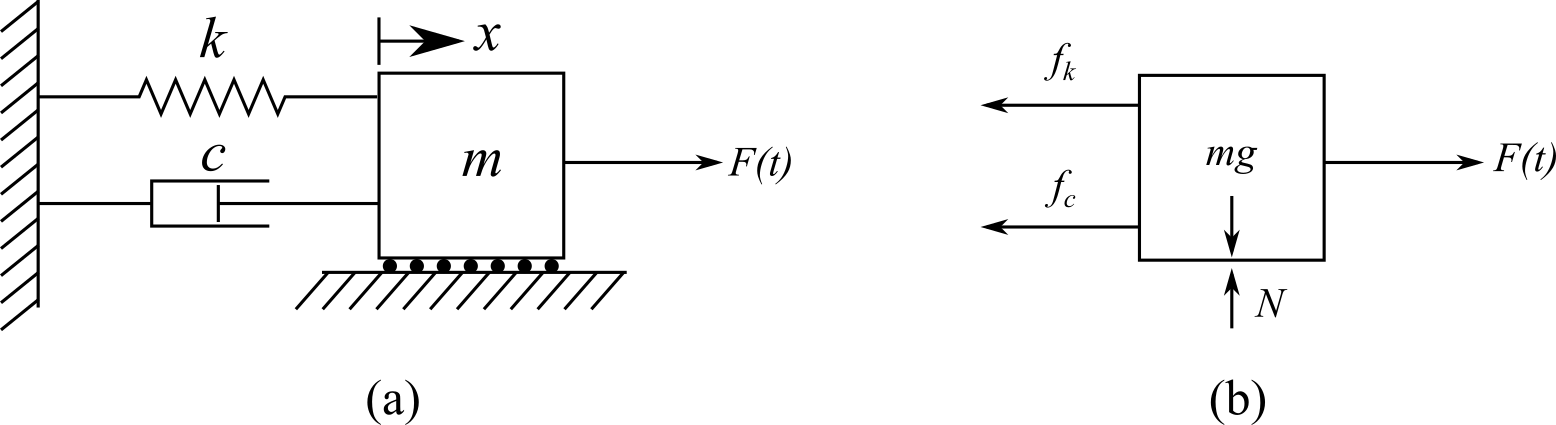
\includegraphics[]{../figures/1-DOF-spring_dashpot_mass_horizontal_forced_FBD.png}
	\caption{Damped 1-DOF system with an external force ($F(t)$) applied, showing: (a) the system configuration; and (b) the free body diagram}
\end{figure}
Newtons second law of motion tells us
\begin{equation}
m \ddot{x} = -kx - c\dot{x} + f^*
\end{equation}
therefore, we can write the EOM as:
\begin{equation}
m \ddot{x}(t) + c\dot{x}(t) + kx(t) = f^*(t)
\label{eq:EOM_2nd_forced}
\end{equation}
for the considered damped forced vibration problem. This is a 2\textsuperscript{nd} order inhomogeneous ODE. As before, the solution of $x(t)$ for equation~\ref{eq:EOM_2nd_forced} is the sum of the complementary and particular solution where the complementary solution satisfies the homogeneous equation while the particular solution satisfies the inhomogeneous equation. 

To solve the homogeneous equation, set the right hand side of equation~\ref{eq:EOM_2nd_forced} to zero to get the equation for damped free vibration:
\begin{equation}
m \ddot{x}(t) + c\dot{x}(t) + kx(t) = 0
\end{equation}
Again, assume $x(t) = Ce^{pt}$, therefore, 
\begin{align}
\dot{x}(t)&= p c e^{ p t}  = px\\
\ddot{x}(t)&= p^2 c e^{ p t} = p^2x \nonumber
\end{align}
Putting these expressions back into the EOM yields:
\begin{equation}
m p^2 x + c p x + k x = 0
\end{equation}
or the characteristic equation
\begin{equation}
mp^2 + c p + k = 0
\end{equation}
solving this expression leads to:
\begin{equation}
p_{1,2} = \frac{-c \pm \sqrt{c^2 -4 m k}}{2 m} = - \frac{c}{2m} \pm \sqrt{\frac{c}{2m} - \frac{k}{m}}
\end{equation}
or:
\begin{equation}
p_{1,2} = - \frac{c}{2m} \pm i \sqrt{\frac{k}{m} - \bigg( \frac{c}{2m}\bigg)^2}
\end{equation}
The critical damping value $c_\text{cr}$ for the system is defined as the value of $c$ that results in a 0 for the radicand (number under the square root). Therefore, we need:
\begin{equation}
\frac{k}{m} - \bigg( \frac{c_\text{cr}}{2m}\bigg)^2 = 0
\end{equation}
\begin{equation}
c_\text{cr} = \frac{k m^2 k}{m} = 4 m k
\end{equation}
this results in:
\begin{equation}
c_\text{cr} = 2  \sqrt{m k}
\end{equation}
The damping ratio $\zeta$ is the ratio between the damping $c$ and the critical damping ratio $c_\text{cr}$, i.e.,
\begin{equation}
\zeta = \frac{c}{c_\text{cr}} = \frac{c}{2 \sqrt{m k}} = \frac{c}{2m\omega_\text{n}}
\end{equation}

Recall that the natural frequency of a system is $\omega_\text{n} = \sfrac{k}{m}$. Damping slightly reduces the natural frequency of the system, resulting in the damped natural frequency $\omega_\text{d}$
\begin{equation}
	\omega_d = \omega_\text{n}\sqrt{1-\zeta^2}
\end{equation} 
Using this expression for the damped natural frequency, the poles of the system can be identified as:
\begin{align}
	p_{1,2} &= - \zeta \omega_\text{n} \pm i  \sqrt{\omega_\text{n}^2 - \zeta^2 \omega_\text{n}^2} \\
&= - \zeta \omega_\text{n} \pm i  \sqrt{1 - \zeta^2} \nonumber \\ \nonumber
&= - \zeta \omega_\text{n} \pm i \omega_\text{d} \nonumber
\end{align}

The damped free vibration response is:
\begin{equation}
	x(t) = c_1 e^{(-\zeta \omega_\text{n} + i \omega_\text{d})t} + c_2 e^{(-\zeta \omega_\text{n} -i \omega_d)t}
\end{equation} 
This simplifies to:
\begin{equation}
	x(t) = e^{-\zeta \omega_\text{n} t} (c_1 e^{i \omega_\text{d}t} + c_2 e^{-i \omega_\text{d}t} )
\end{equation}
or using Euler's equation, 
\begin{equation}
x_\text{c}(t) = C e^{-\zeta \omega_\text{n} t} \sin (\omega_\text{d} t + \phi)
\end{equation}
This equation breaks down into two parts, one for the decay of the system and one for the oscillations as shown below:
\begin{figure}[H]
	\centering
	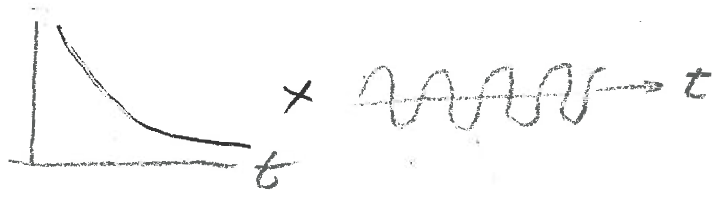
\includegraphics[width=5in]{../figures/decay_and_oscillations.png}
	\caption{Decay and oscillations of the system.}
\end{figure}
Together, these make the free damped vibration response, as computed by the complementary solution $x_\text{c}(t)$
\begin{figure}[H]
	\centering
	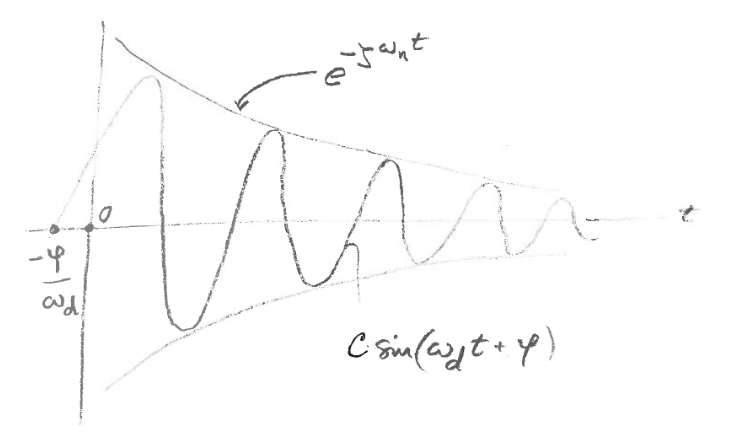
\includegraphics[width=5in]{../figures/free_decay_with_oscillations.png}
	\caption{Free decay with oscillations.}
\end{figure}
Generating the standard form of the damped forced vibration problem is done by dividing the EOM by what leads the first term, mainly:
\begin{equation}
\ddot{x} + \frac{c}{m}\dot{x} + \frac{k}{m}x = \frac{1}{m}f^*(t)
\end{equation}
The expression $\sfrac{c}{m}$ can be rewritten as:
\begin{equation}
\frac{c}{m} = \frac{\zeta c_\text{cr}}{m} = \frac{\zeta 2 \sqrt{m k}}{m} = 2 \zeta \omega_\text{n}
\end{equation}
while the previously defined normalized forcing function is $f(t) = \frac{1}{k}f^*(t)$, this results in a right had side of EOM written as:
\begin{equation}
\frac{1}{m}f^*(t) = \frac{1}{m}kf(t) = \omega^2_\text{n}f(t)
\end{equation}
therefore, the standard form of the EOM for the 1-DOF damped forced vibration problem is written as a 2\textsubscript{nd} order ODE in standard form:
\begin{equation}
\ddot{x} + 2 \zeta \omega_\text{n} \dot{x} + \omega_\text{n}^2 x = \omega_\text{n}^2f(t)
\label{eq:EOM_2nd_order_standard_form}
\end{equation}

The timed resolved solution for the forced vibration problem is:
\begin{align}
\label{eq:x_solution}
x(t) &= x_\text{c}(t) + x_\text{p}(t)  \\
& = e^{-\zeta \omega_\text{n} t } C \sin (\omega_d t + \phi) + x_\text{p}(t) \nonumber
\end{align}
\todo{I don't like the rest of this, why not just use the method of undetermined coefficients?} Putting equation~\ref{eq:x_solution} back into equation~\ref{eq:EOM_2nd_order_standard_form} results in the expression:
\begin{equation}
(\ddot{x}_\text{c} + 2 \zeta \omega_\text{n} \dot{x}_\text{c} + \omega_\text{n}^2 x_\text{c}) + \ddot{x}_\text{p} + 2 \zeta \omega_\text{n} \dot{x}_\text{p} + \omega_\text{n}^2 x_\text{p} = \omega_\text{n}^2f(t)
\end{equation}
where we need to find $C, \; \phi, \; x_\text{p}(t)$ based on the initial conditions of the system. This is not an easy task. 



%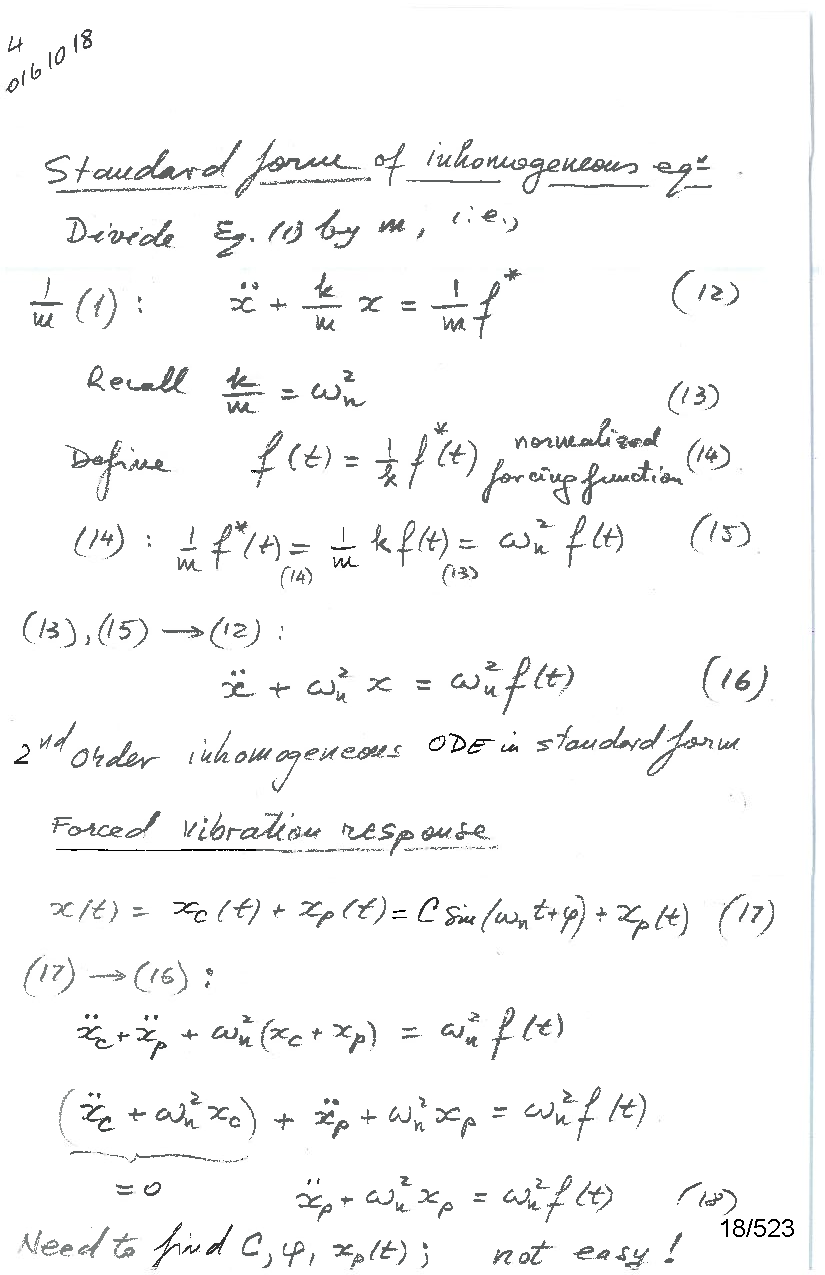
\includepdf[pages=-,pagecommand={},width=0.9\textwidth]{PDF_notes/2nd_order_systems_2.pdf}


\subsection{Stability of 2nd order systems}

Recall that the damped free vibration response:
\begin{equation}
x_\text{c}(t) = C e^{-\zeta \omega_\text{n} t} \sin (\omega_\text{d} t + \phi)
\end{equation}
\begin{figure}[H]
	\centering
	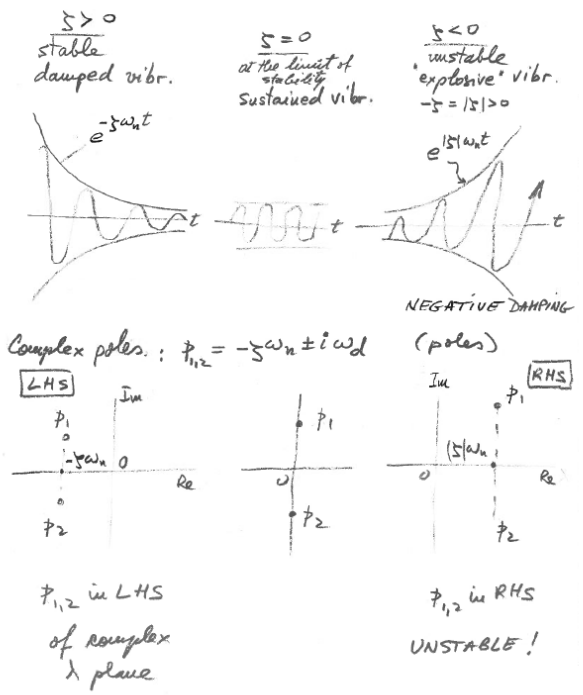
\includegraphics[width=6.5in]{../figures/stability_2nd_order.png}
	\caption{Stability of 2\textsuperscript{nd} order systems.}
\end{figure}

Underdamped, critical-damped, overdamped 2\textsuperscript{nd} order systems and vibration response. 


\begin{equation}
p_{1,2} = -\zeta \omega_\text{n} \pm i  \sqrt{1 - \zeta^2}
\end{equation}

\begin{figure}[H]
	\centering
	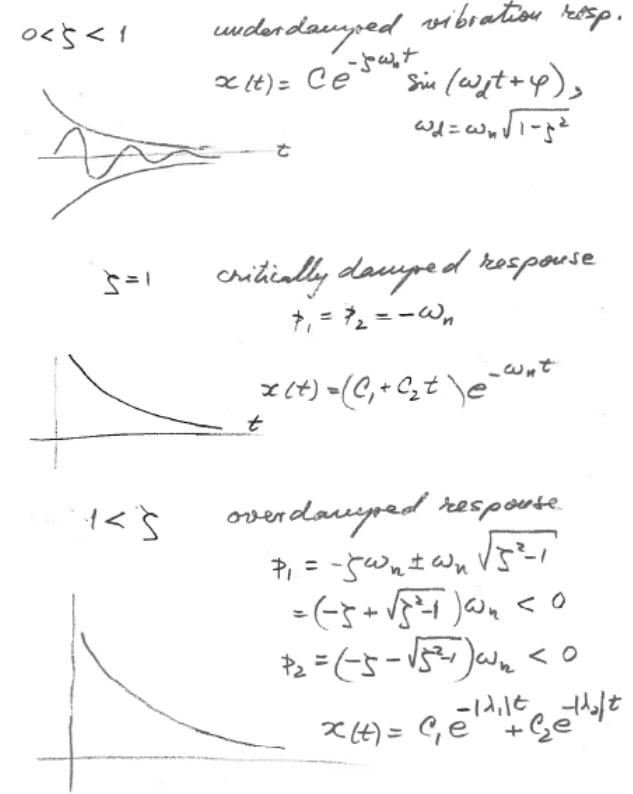
\includegraphics[width=6.5in]{../figures/vibration_responses.png}
	\caption{vibration responses.}
\end{figure}


\begin{figure}[H]
	\centering
	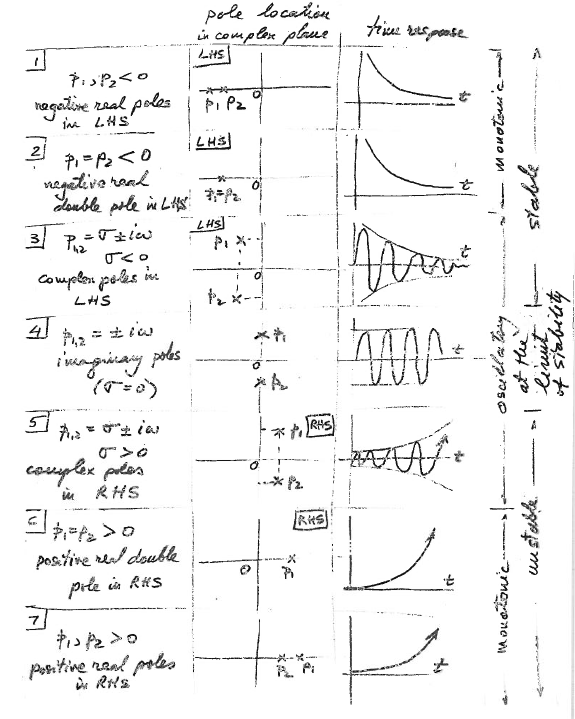
\includegraphics[width=6.5in]{../figures/2nd_order_poles}
	\caption{2nd order poles.}
\end{figure}



\begin{example}
Do example on stability of 2\textsuperscript{nd} order systems
\end{example}

%
%	\pagebreak
%	\renewcommand{\thepage}{}
%	\renewcommand\refname{References Cited}
%	\pagestyle{plain}
%	\bibliographystyle{Downey_NSF}
%	\bibliography{Chapter_1_Basic_Concepts}
%
%
%















\end{document}

